\documentclass{article} 
\usepackage[left=0.75in,top=0.6in,right=0.75in,bottom=0.6in]{geometry} % Document margins
\usepackage{tabularx}
\usepackage{fancyvrb}
%\usepackage[hidelinks]{hyperref}
\usepackage{graphicx}
\usepackage{float}
\usepackage{fancyhdr}
\usepackage{geometry}
\usepackage{lastpage}
\usepackage{tabu}
\usepackage{hyperref}

\geometry{
  top=1in,            % <-- you want to adjust this
  inner=0.5in,
  outer=0.5in,
  bottom=1in,
  headheight=5ex,       % <-- and this
  headsep=4ex,          % <-- and this
}

\pagestyle{fancy}
\fancyhf{}
\rhead{\Large\textit{Old Dominion University}}
\lhead{\Large\textit{ECE 432: Assignment 5}}
\cfoot{Page \thepage \hspace{1pt} of \pageref{LastPage}}
\renewcommand{\footrulewidth}{1pt}

\begin{document}

%----------------------------------------------------------------------------------------
%		 TITLE PAGE
%----------------------------------------------------------------------------------------

\begin{titlepage}

\vspace*{45 pt}
\begin{center}
\Huge{\bf CS 432/532:  Web Science}\\
\huge{Spring 2017\\}

\vspace{60 pt}
\Huge\underline {Assignment 5}\\

\vspace{10 pt}
\Huge{Michael Micros}\\\

{\Large \bf {Instructor: Michael L. Nelson}}\\

\vspace{230 pt}
{\huge \bf {Old Dominon University}}\\
{\huge \bf {Norfolk, Virginia}}\\

\vspace{10 pt}
\today

\end{center}
\end{titlepage}




%----------------------------------------------------------------------------------------
%		PROBLEM 1
%----------------------------------------------------------------------------------------

\section*{{\underline{\huge {Problem 1:}} Predicting the Karate Club split(Zachary,1977)}}

The goal for this assignment was to determine whether it is possible to predict the members of  the 2 groups that formed after the Karate Club split. Based on the data provided in the original paper, an undirected graph can be constructed with each edge representing interactions between members outside of the Karate Club. The idea is that based on these interactions of the members, we can predict  which group each member will belong to after the split, or even if there is a dispute and a split imminent.\\
The data for the experiment was obtained from the UCIrvine Network Data Repository.The specific file is "karate.gml" and can be found at the following URI:\\

 http:// networkdata.ics.uci.edu/data/karate/ \\

The python program ``part1.py'' performs the prediction using igraph's built in algorithm ``community\_edge\_betweenness'', which calculates the betweenness of the edges. The argument ``clusters" specifies how man communities we want after the split, and accordingly the edge or edges with the highest betweenness are cut resulting in the 2 or more factions.\\

In the code, f1 and f2 are the node IDs of the members)  that sided with Mr. Hi and the officer respectively, accoriding to the original paper.

\begin{figure}[H]
 \centering
 	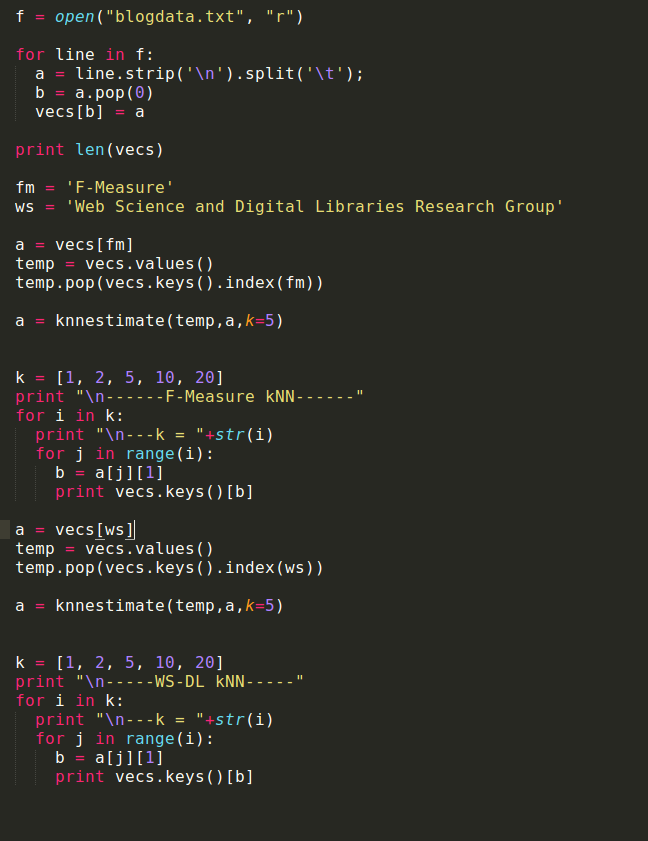
\includegraphics[height=12 cm]{code.png}
  \caption{``part1.py"}
\end{figure}
\newpage

\begin{figure}[H]
 \centering
 	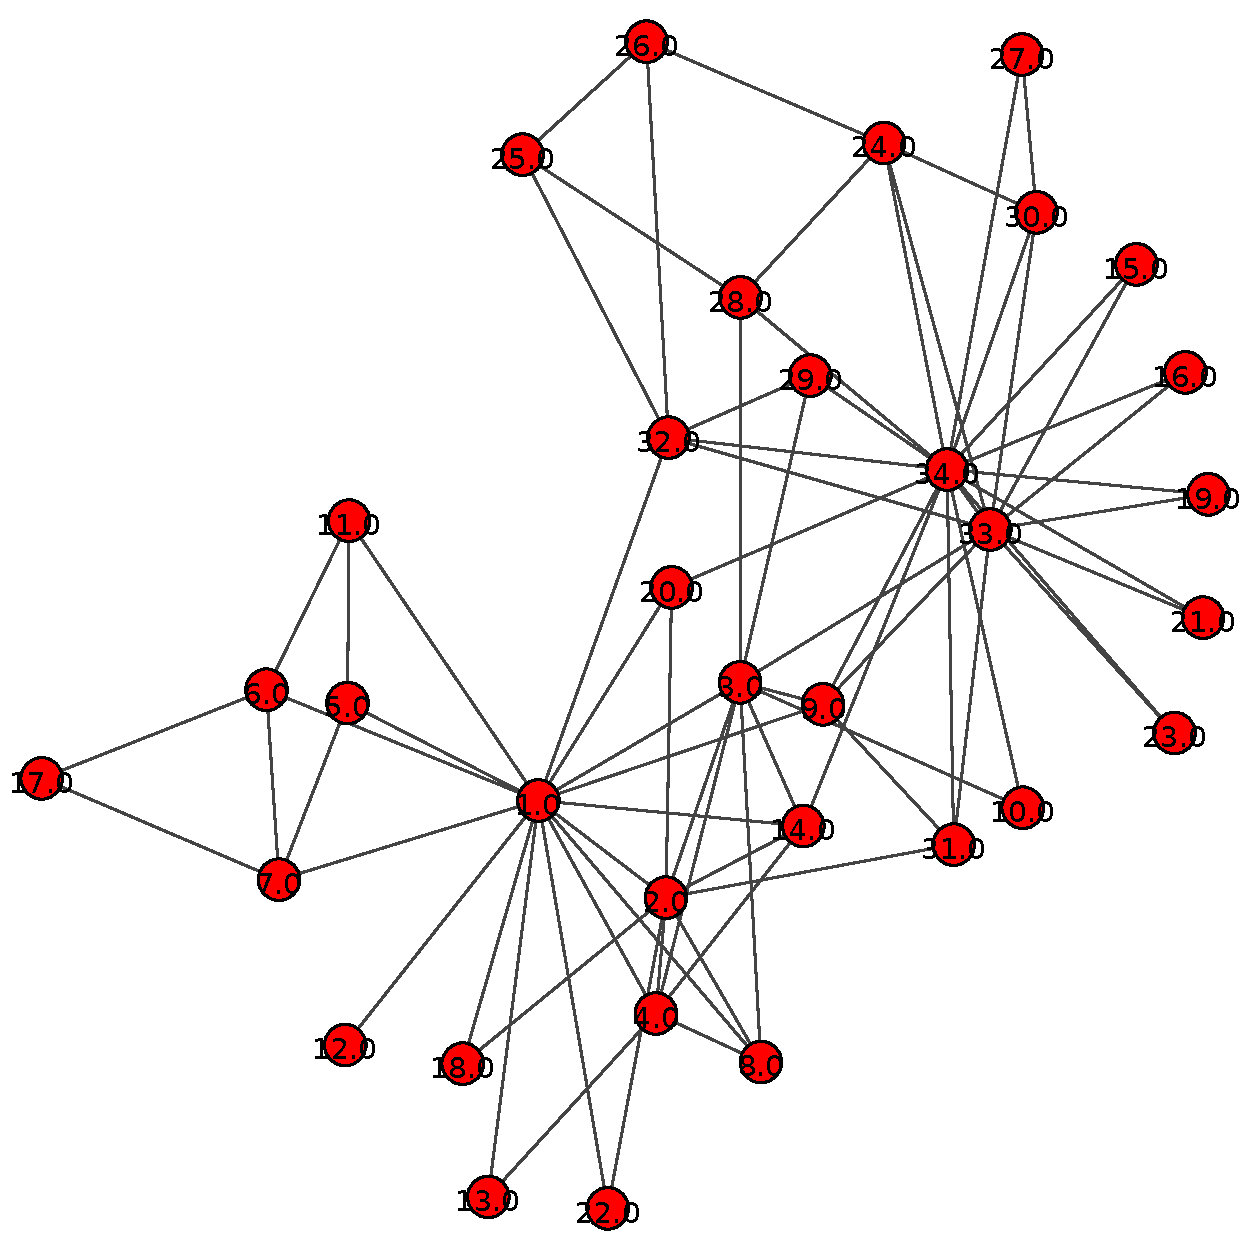
\includegraphics[width=\linewidth]{KarateClub.pdf}
  \caption{Graph of the 34 Karate Club members from the original paper by Zachary}
\end{figure}

\begin{figure}[H]
 \centering
 	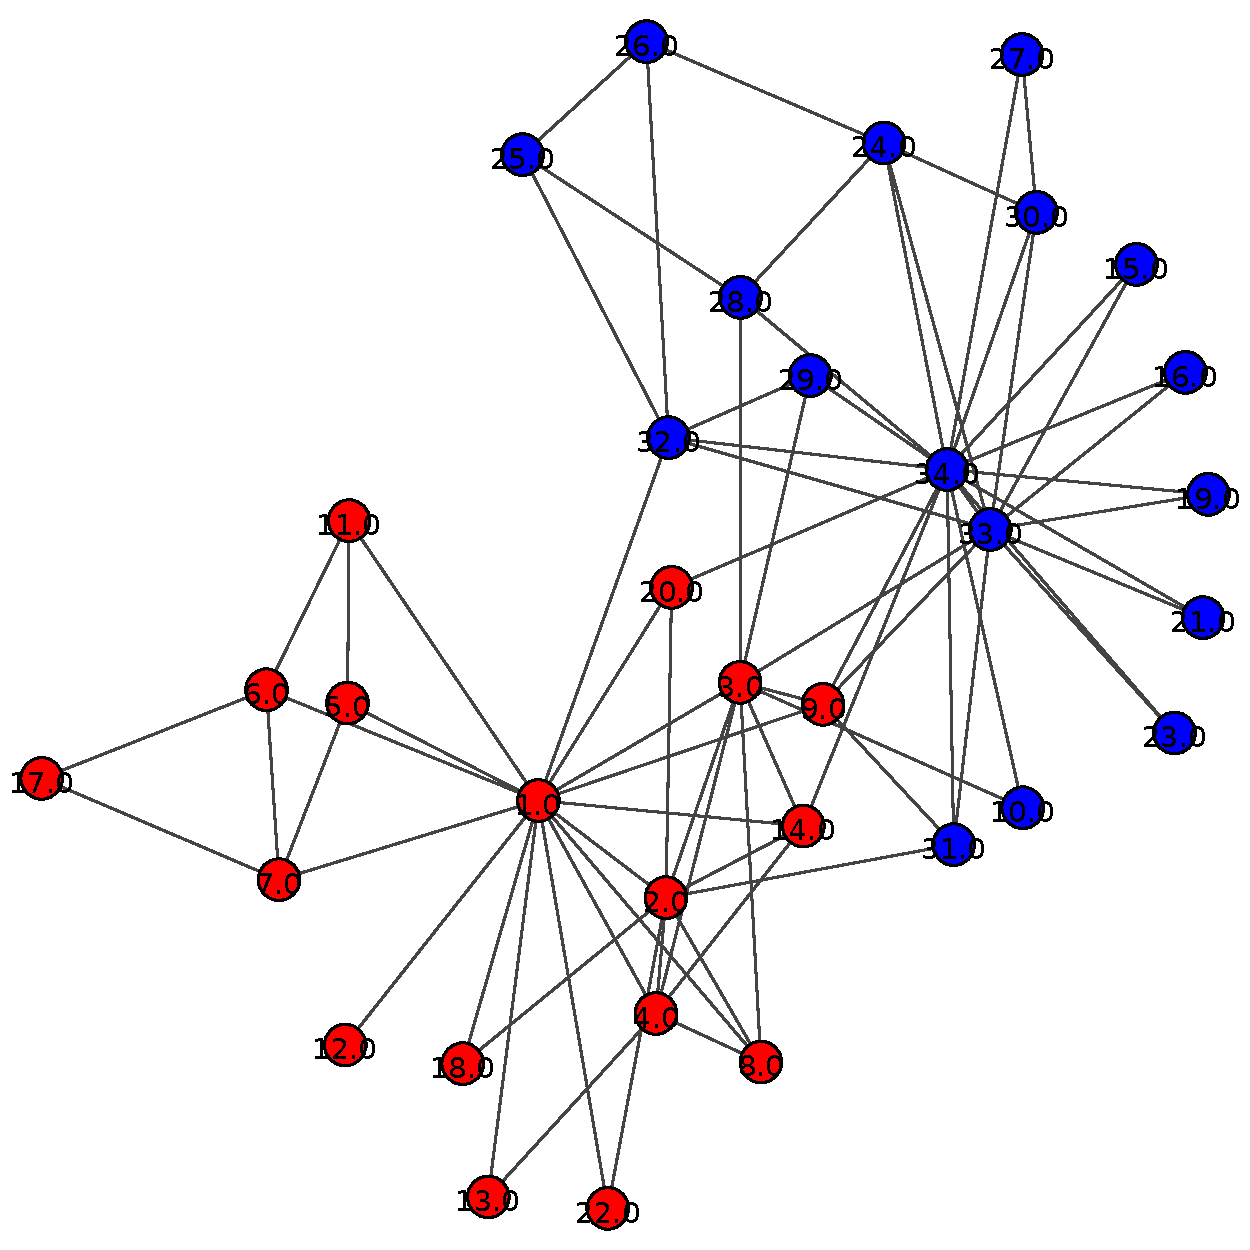
\includegraphics[height=10 cm]{KarateClubFactions.pdf}
  \caption{The 2 groups that formed after the split in the origianl paper.}
\end{figure}

\begin{figure}[H]
 \centering
 	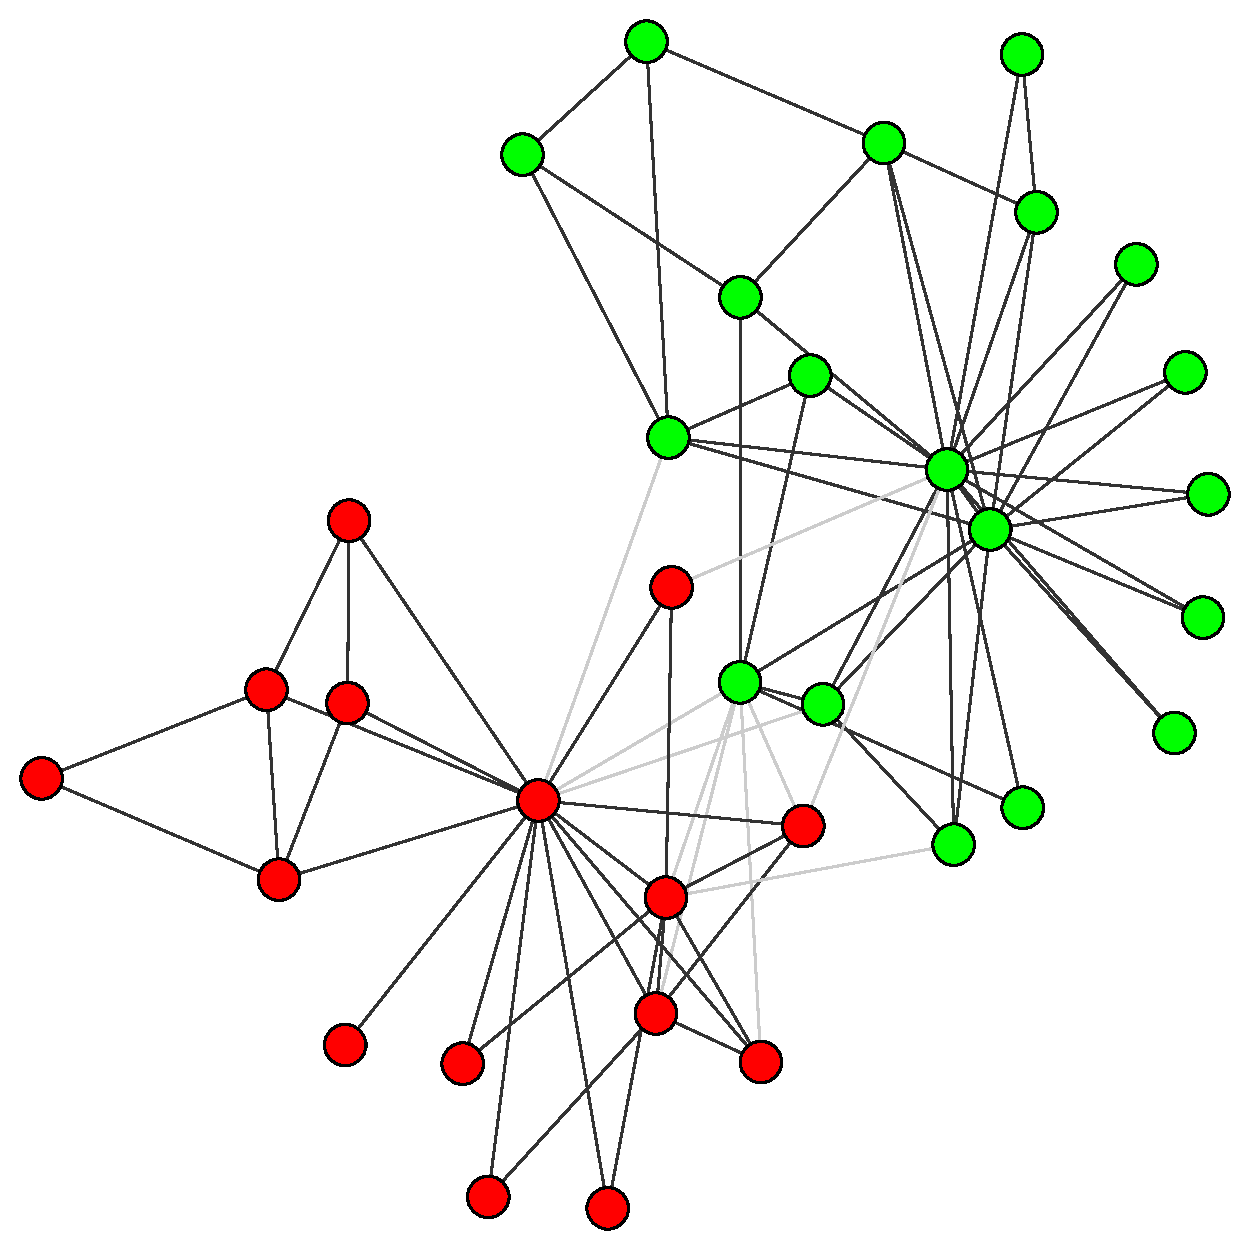
\includegraphics[height=10 cm]{prediction.pdf}
  \caption{The prediction generated by the python script}
\end{figure}

By comparing Figures 3 and 4 it is obvious that the program predicted the final groups right with the exception of members 3 and 9, who had interactions with both groups and it is difficult to say with any certainty to which faction they belonged. That is an accuracy of 0.94, which is acceptable. 


%----------------------------------------------------------------------------------------
\end{document}
